 \let\negmedspace\undefined
\let\negthickspace\undefined
\documentclass[article]{IEEEtran}
\usepackage[a5paper, margin=10mm, onecolumn]{geometry}
%\usepackage{lmodern} % Ensure lmodern is loaded for pdflatex
\usepackage{tfrupee} % Include tfrupee package

\setlength{\headheight}{1cm} % Set the height of the header box
\setlength{\headsep}{0mm}     % Set the distance between the header box and the top of the text

\usepackage{gvv-book}
\usepackage{gvv}
\usepackage{cite}
\usepackage{amsmath,amssymb,amsfonts,amsthm}
\usepackage{algorithmic}
\usepackage{graphicx}
\usepackage{textcomp}
\usepackage{xcolor}
\usepackage{txfonts}
\usepackage{listings}
\usepackage{enumitem}
\usepackage{mathtools}
\usepackage{gensymb}
\usepackage{comment}
\usepackage[breaklinks=true]{hyperref}
\usepackage{tkz-euclide} 
\usepackage{listings}                                       
\def\inputGnumericTable{}                                 
\usepackage[latin1]{inputenc}                                
\usepackage{color}                                            
\usepackage{array}                                            
\usepackage{longtable}                                       
\usepackage{calc}                                             
\usepackage{multirow}                                         
\usepackage{hhline}                                           
\usepackage{ifthen}                                           
\usepackage{lscape}

\renewcommand{\thefigure}{\theenumi}
\renewcommand{\thetable}{\theenumi}
\setlength{\intextsep}{10pt} % Space between text and floats

\numberwithin{figure}{enumi}
\renewcommand{\thetable}{\theenumi}

% Marks the beginning of the document
\begin{document}
\bibliographystyle{IEEEtran}
\title{NCERT-10.3.6.2.3}
\author{EE24BTECH11039 - MANDALA RANJITH}
{\let\newpage\relax\maketitle}


\noindent\textbf{Question: }  
Roohi travels $300$km to her home partly by train and partly by bus. She takes $4$hours if she tarvels $60$km by train and the remaining by bus. If she travels $100$km by train and the remaining by bus, she takes $10$minutes longer. Find the speed of the train and the bus separately.\\\\\
\noindent\textbf{Solution: } 

\begin{align}
    \frac{60}{x} + \frac{240}{y} &= 4 \\
    \frac{100}{x} + \frac{200}{y} &= \frac{25}{6}
\end{align}

\section{Theoretical Solution}
We solve the above equations using elimination:

We get $x=60$ && $y=80$



\section{Numerical Method:}
\section{LU Decomposition to Solve the System}
We now solve the system of equations using LU decomposition.

\subsection{Matrix Form}
The system of equations can be expressed in matrix form as:
\begin{equation}
    \myvec{
    60 & 240 \\
    100 & 200
    } \myvec{x \\ y} = \myvec{4 \\ 25/6}.
\end{equation}
Here, the coefficient matrix is:
\begin{equation}
    A = \myvec
    {60 & 240 \\
    100 & 200}, \quad \vec{b} = \myvec{4 \\ 25/6}.
\end{equation}

\subsection{Step 1: Decomposing \(A\) into \(L\) and \(U\)}
The matrix \(A\) can be decomposed into:
\begin{equation}
    A = L \cdot U,
\end{equation}
where:
\begin{align}
    L &= \myvec{1 & 0 \\ \frac{3}{5} & 1}, \\
    U &= \myvec{100 & 200 \\ 0 & 120}.
\end{align}






\subsection*{Step 2: LU Factorization Using Update Equations}
Given a matrix \( \mathbf{A} \) of size \( n \times n \), LU decomposition is performed row by row and column by column. The update equations are as follows:  

\textbf{Step-by-Step Procedure:}
1. \textbf{Initialization:}  
   - Start by initializing \( \mathbf{L} \) as the identity matrix \( \mathbf{L} = \mathbf{I} \) and \( \mathbf{U} \) as a copy of \( \mathbf{A} \).

2. \textbf{Iterative Update:}  
   - For each pivot \( k = 1, 2, \ldots, n \):  
     - Compute the entries of \( U \) using the first update equation.  
     - Compute the entries of \( L \) using the second update equation.  

3. \textbf{Result:}  
   - After completing the iterations, the matrix \( \mathbf{A} \) is decomposed into \( \mathbf{L} \cdot \mathbf{U} \), where \( \mathbf{L} \) is a lower triangular matrix with ones on the diagonal, and \( \mathbf{U} \) is an upper triangular matrix.  

\subsection*{1. Update for \( U_{k,j} \) (Entries of \( U \))}
For each column \( j \geq k \), the entries of \( U \) in the \( k \)-th row are updated as:  
\[
U_{k,j} = A_{k,j} - \sum_{m=1}^{k-1} L_{k,m} \cdot U_{m,j}, \quad \text{for } j \geq k.
\]
This equation computes the elements of the upper triangular matrix \( \mathbf{U} \) by eliminating the lower triangular portion of the matrix.

\subsection*{2. Update for \( L_{i,k} \) (Entries of \( L \))}
For each row \( i > k \), the entries of \( L \) in the \( k \)-th column are updated as:  
\[
L_{i,k} = \frac{1}{U_{k,k}} \left( A_{i,k} - \sum_{m=1}^{k-1} L_{i,m} \cdot U_{m,k} \right), \quad \text{for } i > k.
\]
This equation computes the elements of the lower triangular matrix \( \mathbf{L} \), where each entry in the column is determined by the values in the rows above it.

\subsection*{LU Factorization of Matrix \( A \)}
We decompose \( A \) as:
\[
A = LU,
\]
where \( L \) is a lower triangular matrix and \( U \) is an upper triangular matrix.  
For the given example, we calculate \( L \) and \( U \) as follows:
\[
L = \begin{bmatrix} 1 & 0 \\ \frac{3}{5} & 1 \end{bmatrix}, \quad 
U = \begin{bmatrix} 100 & 200 \\ 0 & 120 \end{bmatrix}.
\]

\section*{Theoretical Solution using LU Decomposition}

\subsection*{Step 1: Convert to Matrix Form}
Given the equations:
\begin{align*}
    \frac{60}{x} + \frac{240}{y} &= 4 \\
    \frac{100}{x} + \frac{200}{y} &= \frac{25}{6}
\end{align*}
where we define \( a = \frac{1}{x} \) and \( b = \frac{1}{y} \), transforming the system into:
\begin{align*}
    60a + 240b &= 4 \\
    100a + 200b &= \frac{25}{6}
\end{align*}

Rewriting in matrix form:
\begin{equation*}
    A \cdot X = B
\end{equation*}
where:
\begin{equation*}
    A = \begin{bmatrix} 60 & 240 \\ 100 & 200 \end{bmatrix}, \quad
    X = \begin{bmatrix} a \\ b \end{bmatrix}, \quad
    B = \begin{bmatrix} 4 \\ \frac{25}{6} \end{bmatrix}
\end{equation*}

\subsection*{Step 2: LU Decomposition Theory}
LU decomposition expresses the matrix \( A \) as the product of a lower triangular matrix \( L \) and an upper triangular matrix \( U \):
\begin{equation*}
    A = P L U
\end{equation*}
where:
\begin{itemize}
    \item \( P \) is a permutation matrix accounting for row swaps,
    \item \( L \) is a lower triangular matrix,
    \item \( U \) is an upper triangular matrix.
\end{itemize}

For this system, performing LU decomposition yields:
\begin{equation*}
    P = \begin{bmatrix} 0 & 1 \\ 1 & 0 \end{bmatrix},
    \quad L = \begin{bmatrix} 1 & 0 \\ 0.6 & 1 \end{bmatrix},
    \quad U = \begin{bmatrix} 100 & 200 \\ 0 & 120 \end{bmatrix}
\end{equation*}

\subsection*{Step 3: Solve Using Forward and Back Substitution}
We first solve for \( Y \) in:
\begin{equation*}
    L Y = P B
\end{equation*}
where:
\begin{equation*}
    Y = \begin{bmatrix} y_1 \\ y_2 \end{bmatrix},
    \quad P B = \begin{bmatrix} \frac{25}{6} \\ 4 \end{bmatrix}
\end{equation*}

Using forward substitution:
\begin{align*}
    y_1 &= \frac{25}{6} \\
    0.6 y_1 + y_2 &= 4
\end{align*}
Solving for \( y_2 \):
\begin{align*}
    y_2 &= 4 - 0.6 \times \frac{25}{6} = 1.5
\end{align*}
Thus, \( Y \) is:
\begin{equation*}
    Y = \begin{bmatrix} \frac{25}{6} \\ 1.5 \end{bmatrix}
\end{equation*}

Next, solve for \( X \) in:
\begin{equation*}
    U X = Y
\end{equation*}
Using back substitution:
\begin{align*}
    120b &= 1.5 \Rightarrow b = \frac{1}{80} \\
    100a + 200b &= \frac{25}{6}
\end{align*}
Solving for \( a \):
\begin{align*}
    100a &= \frac{25}{6} - 2.5 = \frac{10}{6} = \frac{5}{3} \\
    a &= \frac{5}{300} = \frac{1}{60}
\end{align*}

\subsection*{Step 4: Compute Final Values}
Since:
\begin{equation*}
    x = \frac{1}{a} = 60, \quad y = \frac{1}{b} = 80
\end{equation*}

\textbf{Final Answer:}
\begin{itemize}
    \item Speed of the train = {60 km/h}
    \item Speed of the bus = {80 km/h}
\end{itemize}






\begin{figure}[h!]
   \centering
   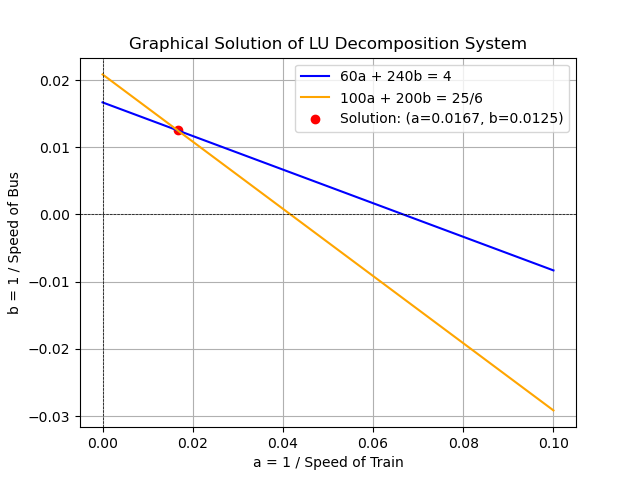
\includegraphics[width=0.8\textwidth]{figures/fig.png} % Ensure this path is correct
   \caption{Plot showing the relationship between  $a$ and $b$}
\end{figure}
\end{frame}



\end{document}


